\chapter{System architecture}

A considerable amount of the project consisted of the actual implementation of the app the team was to deliver to the customer at the end of the semester. 

This chapter provides a detailed description of the app architecture and database structure, and how it was implemented. It also describes how and why said architecture was chosen, and what patterns that were followed in the implementation. 

\section{Architectural overview}
An overview of the architectural components is given in figure~\ref{fig:architecture}. This outline shows the main parts of the current solution. There is a backend server which takes care of storing data to a MySQL database. The app for the time being is implemented on the Android platform and communicates with the server through HTTP with JSON payloads. Section~\ref{sec:arch_design} discusses the overall choices to be made, while section~\ref{sec:arch_app} goes in detail about how the app architecture works. Section~\ref{sec:arch_server} goes in detail about the architecture decisions on the server.

\begin{figure}[H]
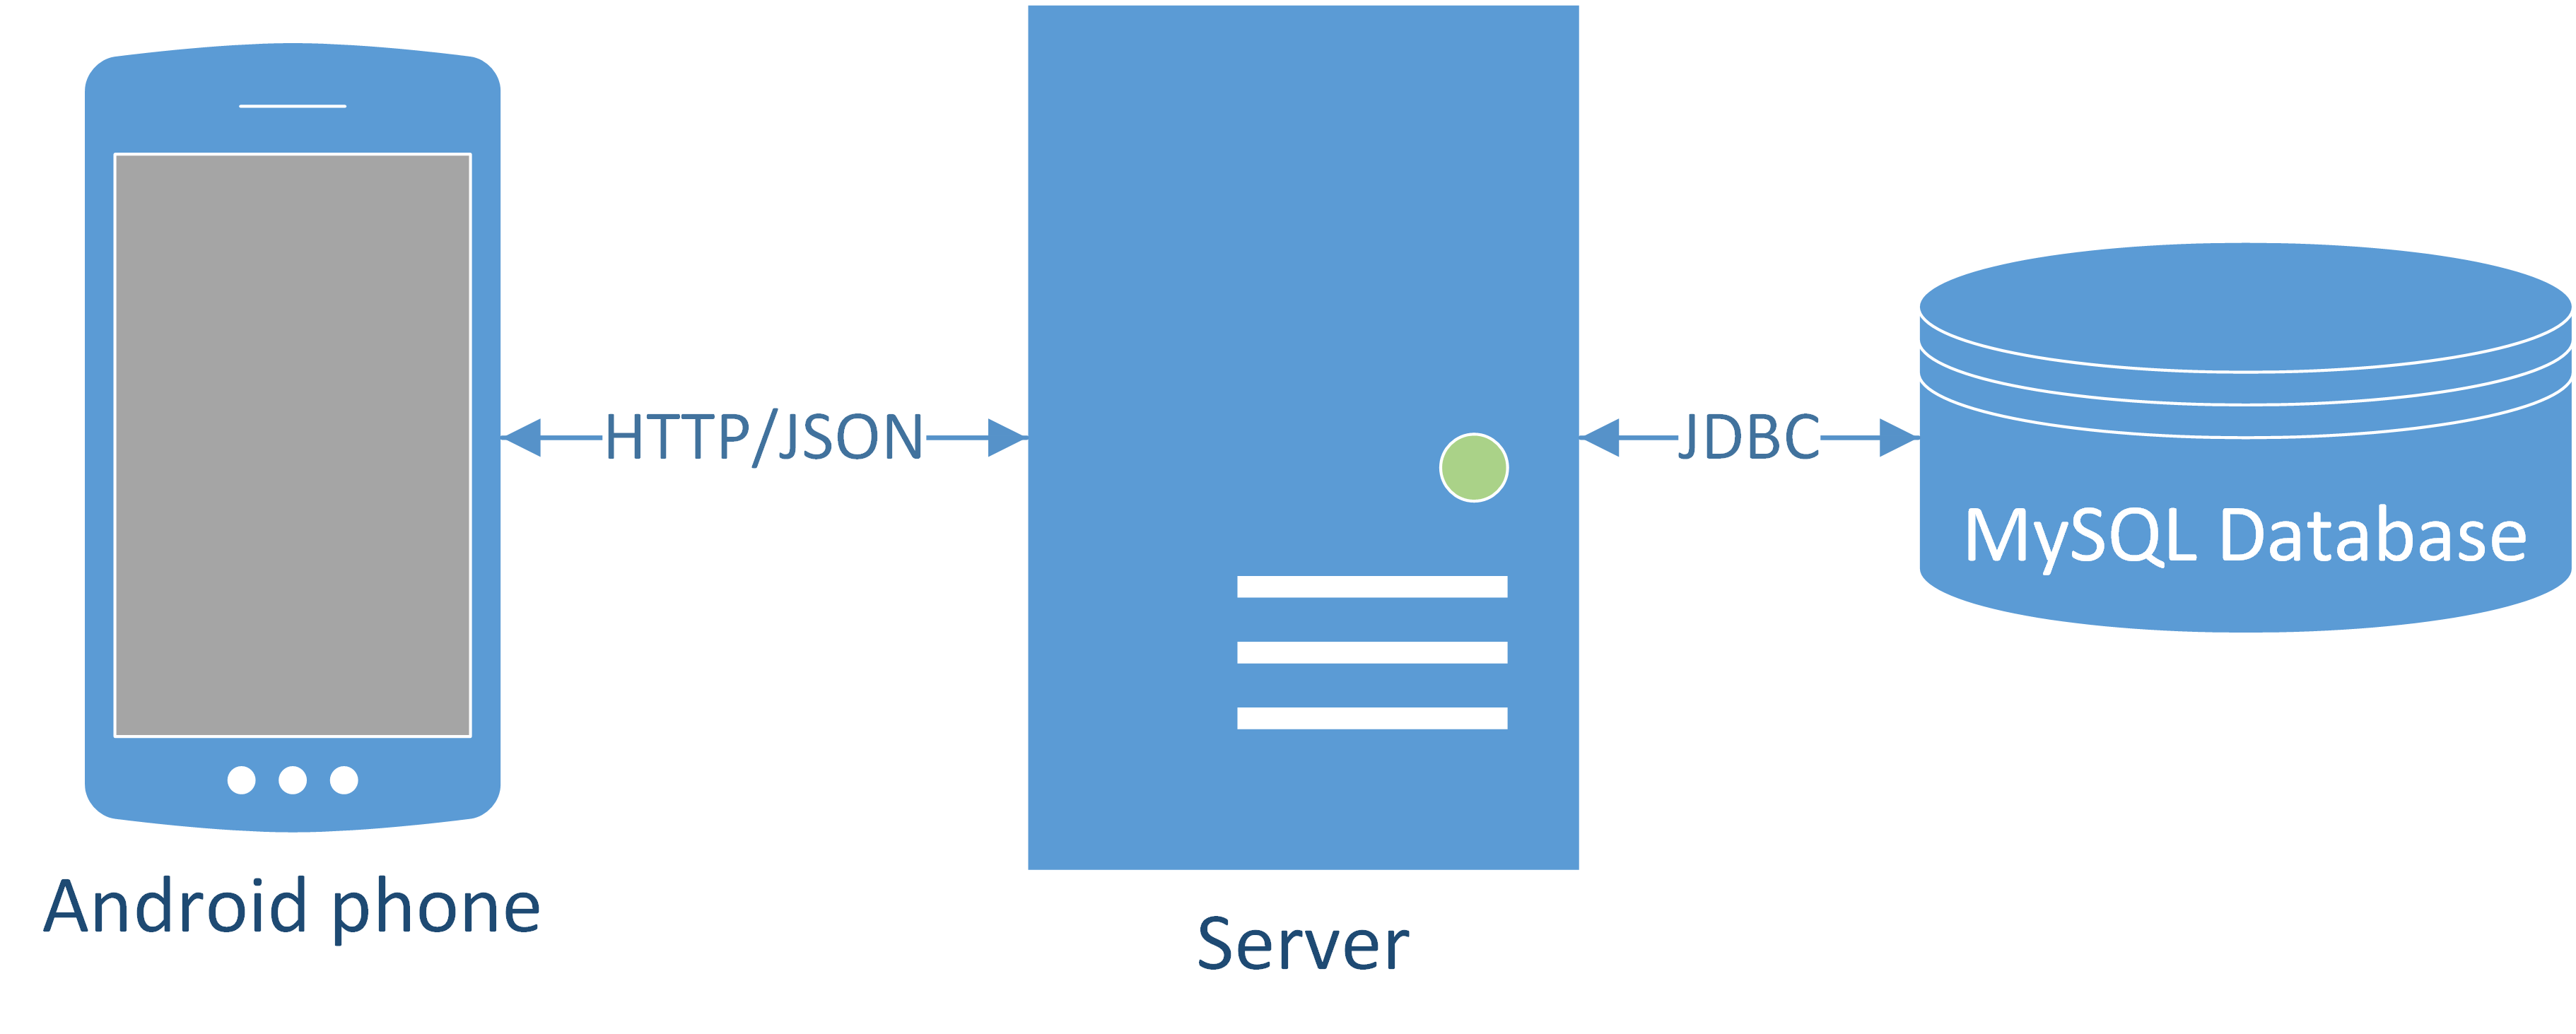
\includegraphics[width=\textwidth]{ch/architecture/fig/arch.png}
\caption{Overall architecture overview.}
\label{fig:architecture}
\end{figure}


\input ch/architecture/sec/design.tex
\input ch/architecture/sec/app.tex
\input ch/architecture/sec/server.tex
